\section{Experiment To Be Conducted}
\textbf{The experiment described in this section are still in the conceptual
  stage, but are planned to be conducted after the detail of implementation is fixed.}

\subsection{Performance Comparison with with User Space Implementation}
It could be achieved without inspecting kernel space to extract the correlation between processes.
For example, one solution was proposed in \cite{Weiqin:ShadowAttack} that
tracks changes to file descriptors in \texttt{/proc/fd} are recorded and subsequently analyzed
every timne a system call related to pipe, socket or file IO operation is executed as shown in \Fref{img:old-method}.
\begin{figure}[tp]
  \begin{center}
    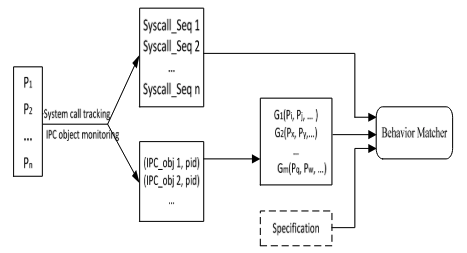
\includegraphics[width=\columnwidth]{./img/old_method.png}
  \end{center}
  \caption{Illustration of architecture of the countermeasure to shadow attacks proposed in
    \cite{Weiqin:ShadowAttack}.}
  \label{img:old-method}
\end{figure}
It should provide some insight about the efficiency of our method to compare the performance of it
with that of user space implementations.

We expect that our method will be more efficient than the user space implementations in the following reasons:
\begin{itemize}
  \item User space approach should confront the large overhead of copying data from kernel space to user space
        \cite{Weiqin:ShadowAttack,jia2023programmable}, but
        in our system that overhead will be mitigated with the efficient data sharing mechanism of eBPF maps.

  \item eBPF can filter out unnecessary information within kernel space before passing it to user space.
\end{itemize}

\subsubsection{Feasibility of Our Method}
We need to evaluate how accurately our method can detect the correlation between processes
while keeping false positive rate low.

For this purpose samples of shadow attack malware have to be prepared. In addition to that,
preparing specification malware detectors is required as the scope of this research is to
efficiently extract the correlation between processes.
